%\section{Uncertainty-aware Network Modeling}
\section{Verification under Uncertainty}
\label{sec:design}

%\wxzc{ to examine consistency during network updates;}

\kevin{We start by describing the problem of network uncertainty (\S\ref{sec:uncertainty}), and then present our solution to model a network in the presence of uncertainty (\S\ref{sec:model} and \S\ref{sec:confirm}).} Our design centers around the idea of \emph{uncertain forwarding graphs}, which compactly represent the entire set of possible network states from the standpoint of packets.
\wxzcr{Next, we describe how we use our model to perform
uncertainty-aware network verification (\S\ref{sec:verify}).}
%\mattc{add a one-sentence roadmap giving the flow of this section}
%We start by introducing the problem of network uncertainty (\S\ref{sec:uncertainty}). We then present \name's uncertainty-aware network model (\S\ref{sec:model} and \S\ref{sec:confirm}).

%, and how to perform network-wide verification using this model (\S\ref{sec:verify}).
%In this section, we describe our design of modeling network state taking uncertainty into account. 

%First, we slice all packets that may enter the network into \emph{equivalence classes} (ECs).
%Each EC is a set of packets that experience the same forwarding actions throughout the network.
%More formally, an EC is defined as:

%\wxzc{Equivalence Class definition, borrowed from veriflow}
%In order to confine our verification activities to only the affected set of packets,
%we slice the network into a set of equivalence classes (ECs) based on the new rule and
%the existing rules that overlap with the new rule. 
%\paragraphb{Definition (Equivalence Class): } An equivalence class (EC) is a set $P$ of packets such that-
%for any $p_1, p_2\in P$ and any network device $R$, the action is identical for $p_1$ and $p_2$ at $R$.

%Next, we model the behavior of packets% belonging to each EC 
%as a graph. 
%Such graphs changes as network states modifications, such as rule additions, removals, or physical failures, happen.
%What is challenging is that from network control point of view, how to model the uncertainty during state transistions?
%Typically, a set of rules in data plane that affect a particular EC is a subset of the entire rule set.
%Similarly, any rule only influence a limited number of ECs in most cases.

%move to implementation
%\subsection{VeriFlow}
%\label{sec:veriflow}
%As the foundation of our work, we first briefly introduce VeriFlow, a real-time network-wide verifier.
%Sitting between the controller and the network, VeriFlow intercept every update issued by the controller before it hits the network and verify its effect in real-time through the following three steps.

%First, VeriFlow slices the entire packet space into a set of Equivalence Classes (ECs) of packets
%using all existing forwarding rules and the new update.
%Each of the ECs is a set of packets that experience the same forwarding actions throughout the network.
%Because each update typically affects a very small number of ECs, 
%to limit searching space,
%VeriFlow only focuses on ECs that might be influenced by the new update. 
%Second, VeriFlow builds a forwarding graphs for each of the affected ECs respectively, 
%representing forwarding behaviors of packets belonging to those ECes.
%Last, VeriFlow traverses each of these graphs,
%to verify network-wide invariants.

\subsection{Network Uncertainty}
\label{sec:uncertainty}

We first describe the problem of network uncertainty and the negative effects of neglecting it.
% on network-wide verification. 
It takes time in networks to disseminate states among distributed and asynchronous devices,
which leads to the inherent \emph{uncertainty} that an observation point
%\cut{tasked with instilling updates consistently into the network, e.g., }
has in knowing the current state of the network. %\kevinc{I prefer to remove the sentence ``which leads to ... by the network".}
We refer to the time period during which the view of the network from an observation point (e.g., an SDN controller)
might be inconsistent with the actual network state as {\em temporal network uncertainty}.
%\mattc{I don't get this sentence -- are you defining "temporal network uncertainty" as a term? If so make it italic and say "Let us refer to the". Or are you defining a quantity here?}. 
The uncertainty could cause network behaviors to deviate from the desired invariants 
temporarily or even permanently. 
%This deviation can affect network verification negatively because of the following two reasons.

%In this section, 
%Here, we define the inconsistency between the view of the observation point and the network state data packets encounter as network uncertainty.

%Network temporal uncertainty imposes a question to network verification: \emph{What if there is uncertainty of the presentation of the network snapshots?}. More specifically, in this paper, we focus on data plane verification by analyzing snapshots of the network-wide data-plane states~\cite{Al-Shaer2009, Al-Shaer2010, VeriFlow, PHA2012, NetPlumber2013}. Before answering this question, we first illustrate how serious the uncertainty can affect network verification.

%First, the bugs caused by such uncertainty, and thus neglected by the current data-plane verifiers, are prevalent.\mattc{I don't see how this paragraph shows they are prevalent. You don't give any statistics about how common they are. Maybe change this into just a motivating example?}
%To illustrate how uncertainty makes the problem much harder,
\if 0
As a motivating example (Figure~\ref{fig:example}), suppose there are two
switches, $A$ and $B$, in the network, and switch $A$ has a forwarding rule
\matt{directing traffic} to switch $B$. 
%\cut{
%For the sake of simplicity,
%\matt{assume this rule causes $A$ to} forward all packets to $B$. 
%}
Now the
network operator wants to reverse the flow of traffic, by making, in sequence,
the following two changes to the network: (1) make switch $A$ remove its
forwarding rule; (2) make switch $B$ insert a new forwarding rule which sends
all traffic to $A$. The network does not contain a loop between $A$ and $B$
before nor after the commands are issued.
However, we do not know exactly when the commands arrive and are processed by
the switches. It is possible that the operation on switch $B$
happens earlier than the one on switch $A$, which results in a transient
loop, leading to increased traffic load as well as lost packets.
%\mattc{I didn't understand the text that was here on "chain of errors" -- how could it cause a chain of errors? What do you mean by chain of errors?}
% the consequence of ignoring such bugs could induce a chain of errors, especially when the transient state lasts sufficiently long. Besides, the example shows that even such a simple and well-planned task can go wrong due to network temporal uncertainty. 
% %Note that in this case, serializing rule installation would help eliminate the bug, but at the cost of performance, and more importantly there are scenarios where carefully crafting ordering doesn't help~\cite{Reitblatt2012}. More devastating examples include errors caused by interleaving between packet arrivals and configuration changes, which will be discussed in more details in Section\ref{sec:motivation}.
% Similar errors can happen in commonly used control programs too. For 
This is not an uncommon--three out of eleven bugs found by NICE~\cite{Nice2012}, 
(BUG V, IX, and XI) are caused by the control programs' lack of knowledge of the network states.

the following two changes to the network: (1) make switch $A$ remove its
forwarding rule; (2) make switch $B$ insert a new forwarding rule which sends
all traffic to $A$.
\fi

\kevin{
Figure~\ref{fig:mt_example} shows a motivating example. Initially, switch $A$ has a forwarding rule
directing traffic to switch $B$. Now the operator wants to reverse the traffic by issuing two instructions in sequence: (1) remove the rule on $A$, 
and (2) insert a new rule (directing traffic to $A$) on $B$. 
%Because of the network uncertainty, 
But it is possible that the second operation finishes earlier than the first one, 
causing a transient loop that leads to packet losses.
That is not an uncommon situation; for example, three out of eleven bugs found by NICE~\cite{Nice2012} 
(BUG V, IX and XI) are caused by the control programs' lack of knowledge of the network states.
}

\begin{figure}[!ht]
  \vspace{-0.1in}
  \centering
  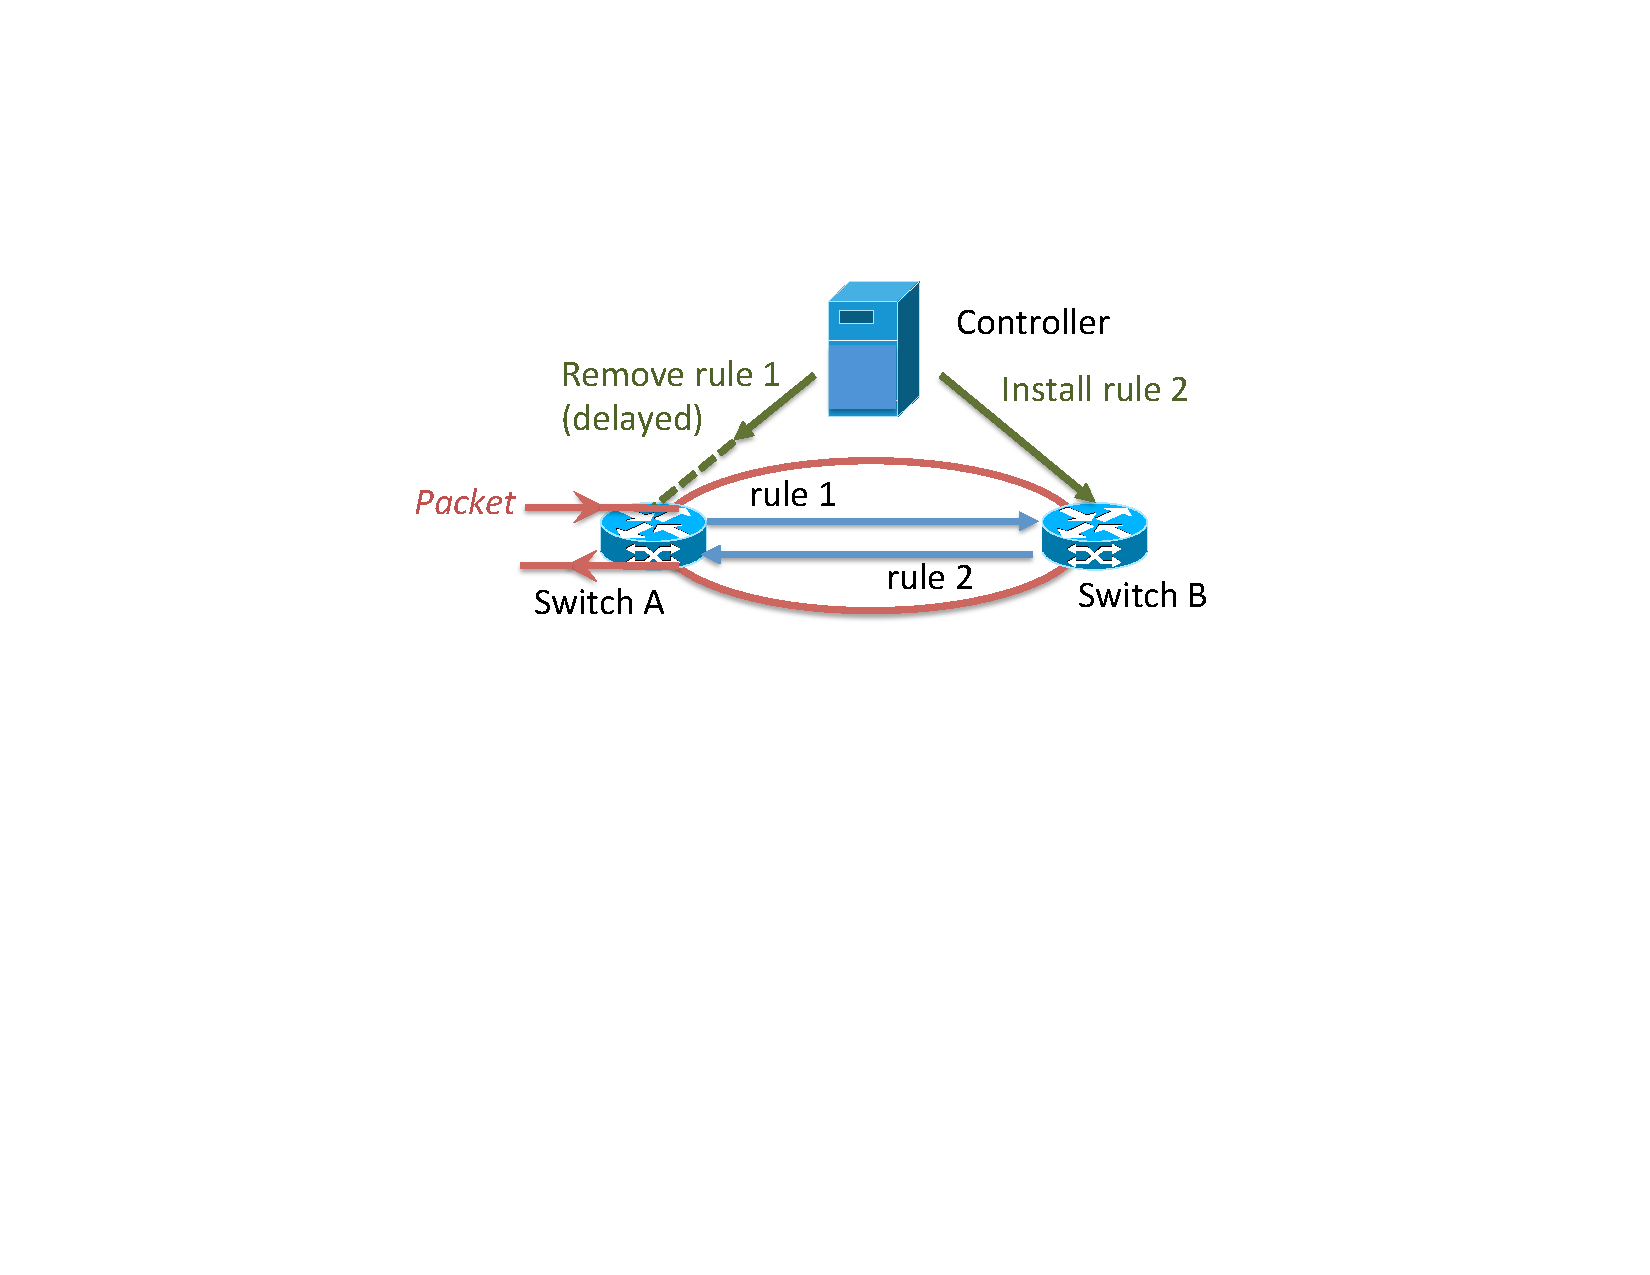
\includegraphics[width=0.7\columnwidth]{figs/example}
  \vspace{-0.1in}
  \caption{\em \small Example: challenge of modeling networks in the presence of uncertainty.}
  \vspace{-0.2in}
  \label{fig:mt_example}
\end{figure}

\if 0
Such errors may have serious consequences.  One may think such uncertainty
related errors are all transient just like the example above.  First of all,
even transient errors can be quite serious.  Take the previous example again.
a packet may enter switch $A$ while the forwarding loop exists. Note that in a
realistic deployment, switches refuse to forward packets back through
their ingress port, but drop them. So the packet will encounter a black hole $B$. 
A recent study~\cite{Flach2013} shows that TCP
transfers with loss may take five times longer to complete compared with
connections with no loss. That is, such bug may cause significant performance
drop. 
%\mattc{I feel like you should move this text up to be at the end of the "First, the bugs caused by uncertainty" paragraph -- that is where you need ot justify this.}
Regarding security issues, for instance, even temporary access control
violations can result in malicious or untrustworthy packets entering a secure
zone~\cite{Reitblatt2012}. 
%Another example is stateful firewall....
%\mattc{I do'nt get the connection bt this sentence and the previous one. Perhaps you are missing a sentence here? Are you giving an example of a temporary access contorl violation? if so why are you talking about performance?}
%\cite{OFCPP}
%\mattc{what is "the early reversing link example"? You mean the example you just gave above? If so just say "example above"}, 
%and thus, ignoring them does not matter much\mattc{don't say that! even transient bugs are very serious! a few milliseconds outage on a terabit link can affect 1000s of connections to majorly back off, harm audio, etc. this sentence weakens your case for no reason -- delete the first part and change the wording to "Even worse,.."}. 
\fi

Such errors may have serious consequences.
\wxznew{In the previous example, the resulting packet losses 
%a packet may enter switch $A$ while the forwarding loop exists,
%and thus gettting dropped there. 
%As switches typically drop packets instead of forwarding them 
%back through their ingress ports, the packet will encounter a black hole at $B$.
%Such errors could cause significant performance drop, e.g., 
could cause a significant performance drop. A recent study~\cite{Flach2013} shows TCP
transfers with loss may take five times longer to complete. 
Other transient errors could violate security policy, e.g., malicious packets could enter a secure zone because of a temporary access control violation~\cite{Reitblatt2012}.}

To make matters worse, errors caused by unawareness of network temporal uncertainty can be permanent. 
For instance, a control program initially instructs a switch to install one rule, and later removes that rule.%then asks the switch to remove that rule.
%The problem is that 
The two instructions can be reordered at the switch~\cite{verified-pldi13}, %so that the switch first removes a non-existing rule, 
\kevin{which ultimately causes the switch to install a rule that ought to be removed.} %resulting a state against the control program's intention. 
%Without querying the flow table at the switch, 
The view of the controller and the network state will remain inconsistent until the rule expires.
One may argue that inserting a barrier message in between the two instructions would solve the problem. 
%However, realistic cases are much more complex than this simple demonstrative example. 
%While in this case, serializing the rule installation would help eliminate the bug at the cost of performance, \mattc{don't imply things indirectly like this, it's confusing. say explicitly "
%However, serializing rules with barrier messages 
However, this may harm performance \kevin{because of increasing control traffic \wxznew{and switch operations}.} %increasing delays and control traffic. 
There are also scenarios in which carefully crafting an ordering does not help~\cite{Reitblatt2012}. In addition, %there is another question of %who should be responsible to discover this problem and to insert the barrier message.\mattc{I don't udnerstand this sentence -- isn't the controller the only option here? Maybe you mean , there's a question of 
%how the controller is able to figure out when to insert the messsages. 
\kevin{it is difficult for a controller to figure out when to insert the barrier messages.}
\name addresses that by \wxznew{serializing only updates that have potential to cause 
race conditions that violate an invariant} (\S\ref{sec:impl}).
%\mattc{btw does your algorithm help with this? If so, mention that as a possible nice use of your alg}
%\kevin{ repeated sentence: As for commonly used control programs, things are the same. 
%Three out of eleven bugs found by NICE~\cite{Nice2012}, (BUG-V, BUG-IX, and BUG-XI) are caused by the control programs' lack of knowledge of the network sate. } 

%Moreover, even if the errors disappear after a while, they could have negative impact on networks in terms of both security and performance. 
%Moreover, even transient errors can be quite serious.
%performance
%security
%An example of security issues includes 
%
%To illustrate how many potential bugs are missed when network uncertainty is neglected\mattc{This is really indirect. How about something like "
%\cut{
%Unfortunately, many SDN applications do not explicitly take into account this uncertainty. For example, network verification tools such as Veriflow assume a zero propagation delay between the controller and the network, which can lead to incorrect results. To evaluate this, we conduct measurement study, and results are shown in \S\ref{sec:bug-coverage}.
%}
%to illustrate how many potential bugs are missed if network uncertainty is neglected
%can cause performance drop. 
%in \S\ref{sec:bug-coverage}. 

\subsection{Uncertainty Model}
\label{sec:model}


%matt's comment{VF doesn’t deal with time. take into account delay, reordering.
%Control asymmetry, symbolically. Time dependent...}

%Although VeriFlow incrementally verifies the network when there are changes, and does so in real-time,



%First, using the new rule and any overlapping existing rules, we slice the network into a set of equivalence classes (ECs) of packets.

%As discussed previously, existing network verification tools do not take into account of the controller's uncertainty of the network state. But the fact is, 

%\mattc{This section starts too abruptly. when I get to this poitn I have no idea what this section is about or what you're goign ot show. Add a 1-2 sentence description of what this sec is about. Also you just jump into describing what the model is without talking about why you need a model (eg "
%To address the problem, we construct a model that accurately represents the controller's uncertainty about the network state.
%\cut{, along with a checking process to allow the controller to make decisions on when and how to send updates by checking that model. %We start by presenting the modeling technique.
%}

%For every update, assuming the controller is able to figure out whether the update is applied in the network after issuing it, there is a period of time during which the controller is uncertain about the state of the network. 

\wxzcr{
We first briefly introduce our prior work VeriFlow, a real-time network-wide verifier.
VeriFlow intercepts every update issued by the controller before it hits the network and 
verifies its effect in real-time.
VeriFlow first
slices the entire packet space into a set of Equivalence Classes (ECs) of packets
using all existing forwarding rules and the new update.
Each EC is a set of packets that experiences the same forwarding actions throughout the network.
%Because each update typically affects a very small number of ECs, 
%to limit searching space,
%VeriFlow only focuses on ECs that might be influenced by the new update. 
Next, VeriFlow builds a forwarding graph for each affected EC
by collecting forwarding rules influencing the EC. 
%representing forwarding behaviors of packets belonging to those ECes.
Lastly, VeriFlow traverses each of these graphs,
to verify network-wide invariants.
}

Naively, to model network uncertainty, for every update, we need two graphs to symbolically represent the network behavior with and without the effect of the update for each influenced EC, until the controller is certain about the status of the update.
%With that approach, 
If $n$ updates are concurrently ``in flight" from the controller to the network, we would need $2^n$ graphs to represent all possible sequences of update arrivals.
%Then, \kevin{\wxznew{when} \cut{for} $n$ updates concurrently ``in flight'' from the controller to the network, \wxznew{to represent} all possible sequences of update arrivals requires \cut{us to maintain} $2^n$ graphs. 
Such a state-space explosion will result in a huge memory requirement and excessive processing time to determine consistent update orderings.
%In addition, we would like to use this model to derive an algorithm to determine consistent update orderings -- executing query algorithms atop such a large amount of state would be excessive.
%, and the query time also grows proportionally. 
%Moreover, it will be really hard for operators to query possible errors in the network at any time instant with the naive approach.\wxzc{repeated errors, hard to interpret} \mattc{I don't understand the last sentence -- what do you mean by repeated errors? Why would multiple graphs be hard to interpret -- seems easier to understand than the symbolic thing you end up with in this section}

%to figure out what might go wrong.
%Therefore, we need a more efficient way to represent all possible forwarding behaviors under uncertainty. 
To address that, we efficiently model the network forwarding behavior %of each EC 
as a \emph{uncertain forwarding graph}, in which links can be marked as {\em certain} or {\em uncertain}.
%\mattc{shouldn't "rules" not "links" be uncertain? In fact, shouldn't uncertainty be a property for both?}
%\mattc{You never said explicitly what uncertain links are, let me add it:}
A forwarding link is {\em uncertain} if the controller does not yet have information on whether 
that corresponding update has been applied to the network.
%\cut{state yet or not}.
%\mattc{There are a lot of things here you're leaving implicit -- need to make sure reader has a complete understanding of your system, let me add:}
The graph is maintained by the controller over time. 
When an update is sent, its effect is applied to the graph and marked as uncertain.
After receipt of an acknowledgment from the network that an update has been applied
% \cut{processed by the switch} 
(or after a suitable timeout%\cut{if the SDN does not support ack'd updates}
), the state of the related forwarding link is changed to {\em certain}.
Such a forwarding graph represents all possible combinations
of forwarding decisions at all the devices.
%By inspecting the graph, the controller becomes aware of which states 
%in the network are reliably known, whether a newly arrived update from an application could result in an inconsistency with in-flight updates, and so on.

\if 0
One complication is that routers maintain multiple forwarding rules, each of which can affect
different subsets of packets. Hence, representing uncertainty on the granularity of
 physical links is not sufficient; an update may affect only one subset of packets traversing a link. Therefore, \name maintains a {\em set} of uncertainty graphs. To minimize the number of graphs we need to store,
we maintain only one graph per {\em equivalence class}, i.e., per each set of packets that undergo the same forwarding behavior 
throughout the network. Our notion of equivalence classes is similar in spirit to those used by HSA and VeriFlow, but applied to our uncertainty graph.
%\mattc{did I get this right? or do you just maintain one graph and have links for each EC?}

%We assume that there exists some mechanisms to get feedbacks from the network to confirm each controller-issued update, and the details will be discussed in \S~\ref{sec:impl}. \name stores all the possible forwarding rules in the data plane, 
%including rules that are supposed to be deleted or replaced by previously issued control messages, 
%but the deletion or replacement has not yet been confirmed, and the corresponding forwarding rules are stored as \emph{uncertain} rules. 

%When rules are collected from each device to construct a forwarding graph, 
%\name usually gets more rules compared with models that do not consider uncertainty
%\mattc{I think you should say "
%\cut{It is important to }Note that although the size of the uncertain graph could still 
%be larger than approaches that simply store a snapshot of the network,
%" -- then say why like you do below. Then at the end, poitn out "
%\cut{However, in practice, the size of this graph} 
%it is far less than storing all possible network states explicitly.
Note that it takes much less space to store the uncertainty graph than to store 
all possible network states explicitly, although it still takes more space than 
would be needed simply to store a static snapshot of the network.
%\kevin{Note that the size of the uncertain graph is far less than storing all possible network states explicitly,
%\wxznew{although it is still larger than simply storing a static snapshot of the network. }
%For example, in the OpenFlow protocol, each rule is associated with a pattern of packet header, actions to handle packets that match the pattern, and a priority to disambiguate between overlapping patterns. 
For example, an OpenFlow device typically handles an incoming packet with the highest-priority rule that the packet header matches.
%Accordingly, without considering uncertainty, %for packets of a particular pattern, the forwarding graph only takes the highest priority rule that matches that pattern at each node.
%\cut{Therefore in the graph, each node has no more than one outgoing link.}
\name collects not only the rule with the highest priority, but also the rules from the highest priority to lower priorities until a \emph{certain} rule (included) is found. This is because any rule in this collection may be used to forward packets at the moment.
%In other words, because of uncertainty, some nodes have more than one outgoing links, among which up to one is certain.
\fi

In this way, the extra storage required for uncertainty modeling is linearly bounded by the number of uncertain rules.
%, and so is the query time (\S\ref{sec:verify}). The reason is that in the worst case, there are $n$ parallel paths that need to be traversed, %instead of one without considering uncertainty, 
%where $n$ is the number of concurrent uncertain rules.
We next examine ``garbage collecting'' states from the graph, i.e., when one can confirm links as certain.
%That leads to the question of when it is possible to ``garbage collect'' state from the graph, i.e., when one can ``confirm'' links as being certain (\S\ref{sec:confirm}). \cut{We describe this issue in the next subsection.}

\begin{figure}[!ht]
  \centering
  \vspace{-0.1in}
  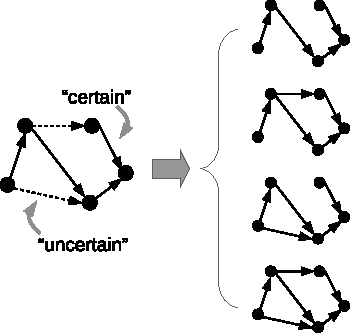
\includegraphics[width=0.6\columnwidth]{figs/model2}
  %\vspace{-0.2in}
  \vspace{-0.15in}
  \caption{\em \small \name's uncertain forwarding graph. 
%symbolic network representation provides a compact way to represent the uncertainty in a monitored network state.
  %\mattc{make this figure smaller. I feel like the size highlights it too much, it's enormous}
  }
  \vspace{-0.2in}
  \label{fig:model}
\end{figure}

\subsection{Dynamical Updating of the Model}
\label{sec:confirm}

\matt{
In order to model the most up-to-date network state, we need to update the model as changes happen in the network.
At first glance, one might think that could be done simply by marking forwarding links as uncertain when new updates are sent, and then, when an ack is received from the network, marking them as certain.
%However, \cut{there is a tricky case we need to take into account.}
%the challenge is we also need to model data packets in the network:
%\cut{In particular, the problem is that}
The problem with that approach is that it may result in inconsistencies from the data packets' perspective}
%, e.g., even after a switch removes a rule, packets that had been processed by that rule might remain in flight.}
Consider a network consisting of four switches, as in Figure~\ref{fig:filtermoving}. %consisting of four switches operated by an SDN controller, $s_1-s_4$ (Figure~\ref{fig:filtermoving}).
%\cut{It is important to take into account these packets as well, as not doing so could introduce inconsistency issues.} \cut{-- for example, a new update installed with the assumption that all data in flight in the network is processed with existing rules could misroute or drop these existing packets, as it would not expect them to be in flight.}


%Besides modeling uncertainty with limited space, choosing a proper timing\mattc{I thought you don't use timign -- I thought you used explicit ack'ing? Maybe just say "space, determining when to confirm uncertain..."} to confirm uncertain updates is challenging too. 

%Intuitively, one may think that it is safe to change the tag of a stored rule from uncertain to certain when the feedback from the network is received at the controller. We first illustrate why that intuition is incorrect with the following example. 

\begin{figure}[!ht]
  \centering
  \vspace{-0.15in}
  %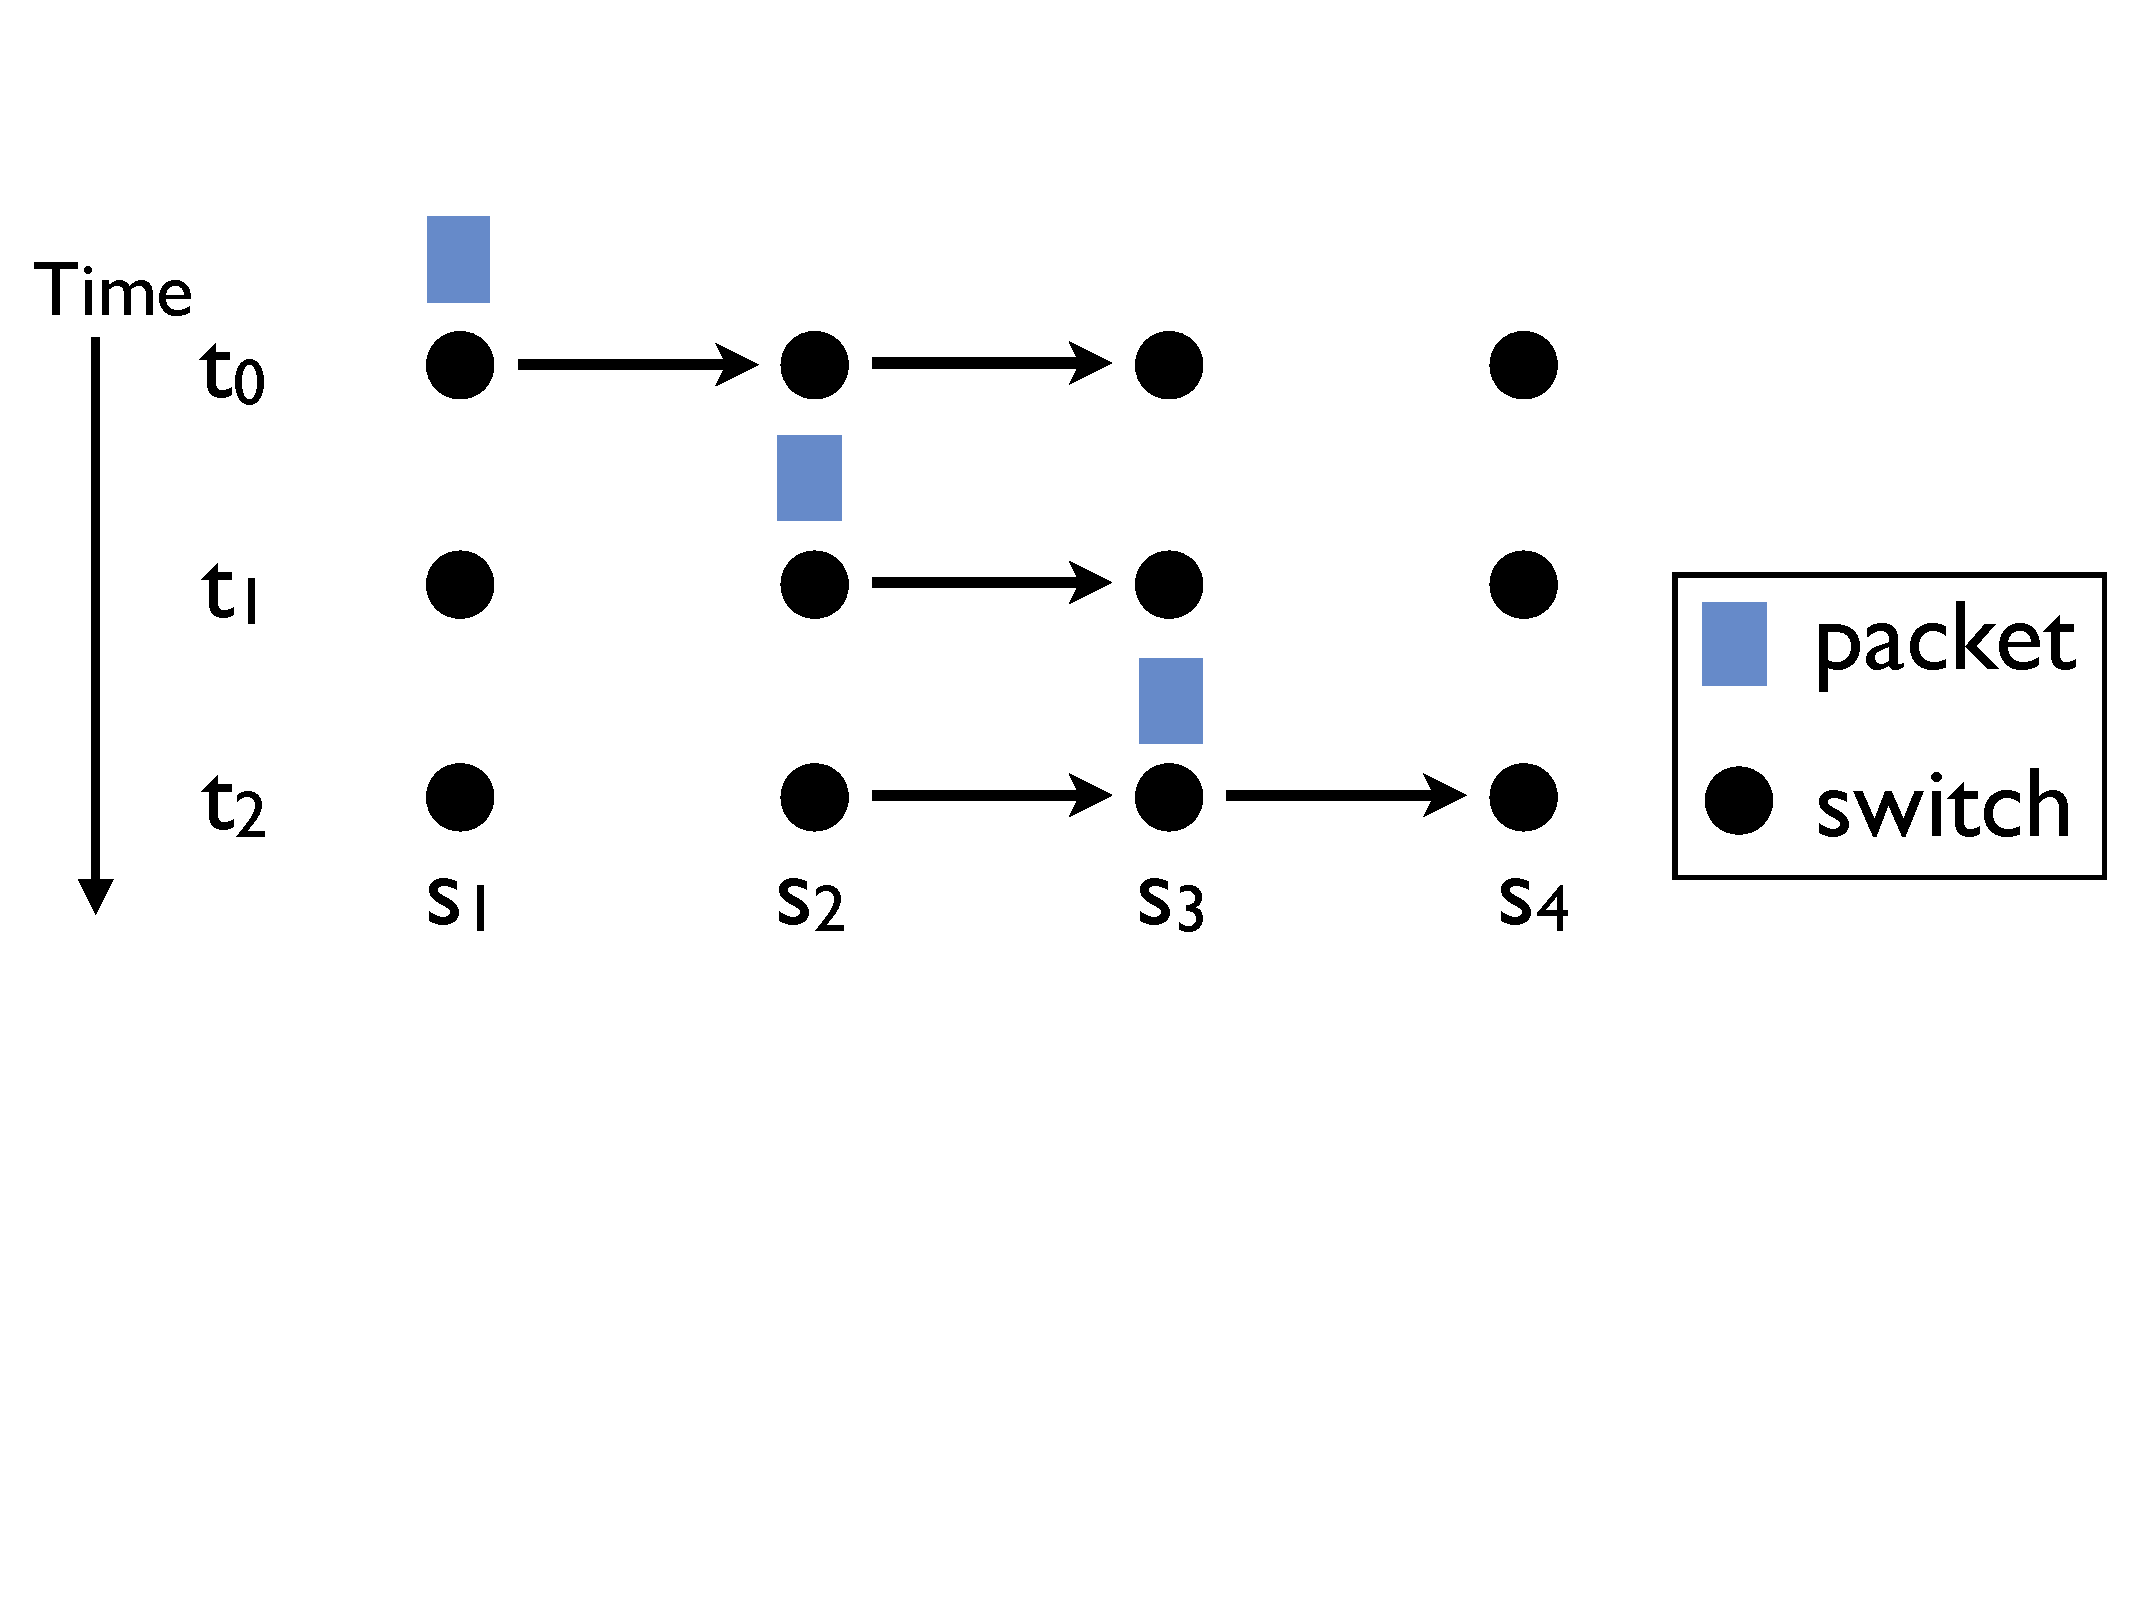
\includegraphics[width=2in]{figs/filtermoving}
  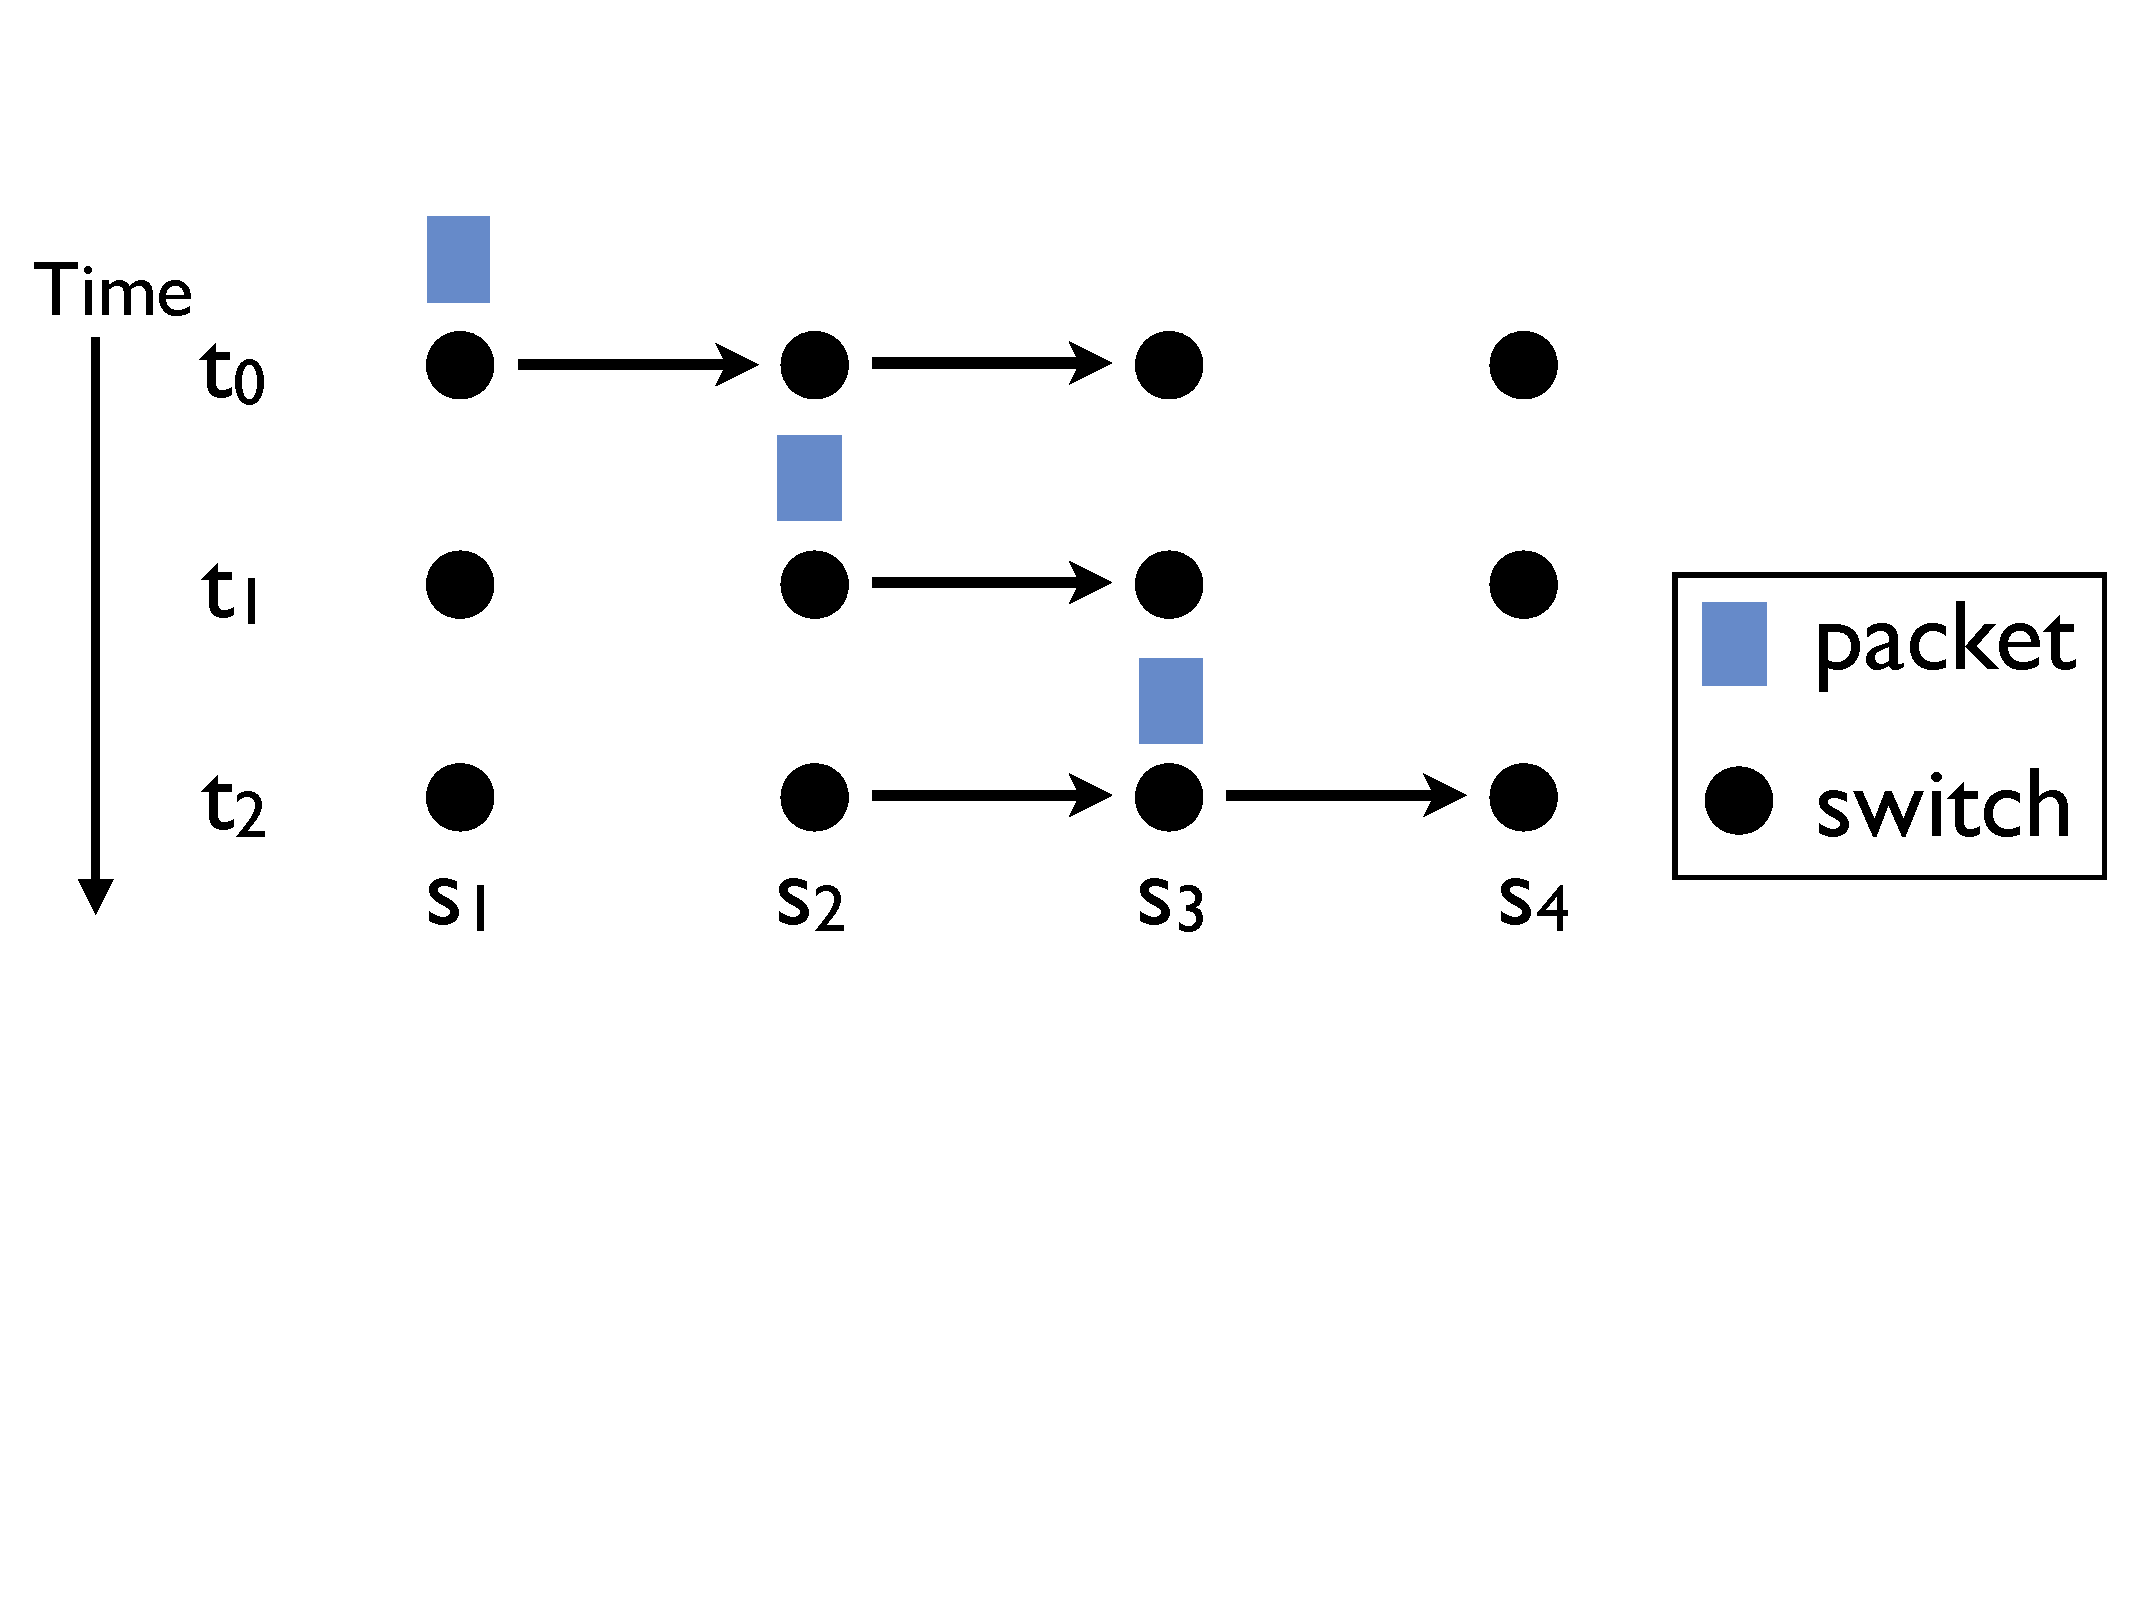
\includegraphics[width=0.8\columnwidth, trim=0mm 0mm 0mm -2mm]{figs/filtermoving}
  \vspace{-0.1in}
  \caption{\em \small Example: challenge of dealing with non-atomicity of packet traversal.}
  \vspace{-0.2in}
  \label{fig:filtermoving}
\end{figure}

%- when an ack comes back I don't process it yet - bc there's packets in flight

%\cut{To illustrate this in more detail,} 
%Let us 
The policy to enforce is that packets from a particular source entering Switch $s_1$ should not reach Switch $s_4$.
Initially, at time $t_0$, Switch $s_3$ has a filtering rule to drop packets from that source, 
whereas all the other switches simply pass packets through.
The operator later wants
%\cut{to change the configuration} 
to drop packets on $s_1$ instead of $s_3$.
%\cut{ at time $t_2$.} 
%Apparently, both the initial and final states preserve the policy.
To perform the transition in a conservative way, the controller first adds a filtering rule on $s_1$ at $t_1$, then removes the filtering rule on $s_3$ at $t_2$, after the first rule addition has been confirmed.

%Each of the forwarding graphs seems correct. 
\kevin{The forwarding graphs at all steps seem correct.}
However, if a packet enters $s_1$ before $t_1$ and reaches $s_3$ after $t_2$, 
it will reach $s_4$, which violates the policy.
%\mattc{delete the exclamation point, and add text here saying explicitly "
\wxzcr{Traversal of a packet over the network is not atomic, 
interleaving with network updates,
as also observed in~\cite{Reitblatt2012}. 
Moreover, it is recently proved that there are situations where no correct update order exists~\cite{bad-pkts}.}
%Note that we are not the first to observe that problem~\cite{Reitblatt2012}.
To deal with it, upon receiving an ack from the network, \name does not immediately mark the state of the corresponding 
forwarding link as certain.
Instead, it delays application of the confirmation to its internal data structure. 
In fact, confirmations of additions of forwarding links in the graph model can be processed immediately, and only confirmations of removals of forwarding links
%\cut{in the graph model} 
need to be delayed. 
The reason is that \wxzcr{we want to ensure we represent all the possible behaviors of the network.} 
Even after a forwarding rule has been deleted, packets processed by the rule may still exist in the network, buffered in an output queue of that device, in flight, or on other devices. %That is, there are packets have this rule's footprint in their history, and for these packets, their view of the network state contains this rule throughout their lifetime in the network.
%Such confirmations include acknowledgments of deletion, expiration, or replacement by a higher-priority rule on the same device.
%\cut{
%Note that some in-flight packets handled by those forwarding links may still exist in the network. For those packets, their views of the network contain a subset of those non-existing links. }

%\cut{To decide that}
%As for how long confirmations should be delayed, 
%\wxzcr{as in past work~\cite{Reitblatt2012, incremental-cu}},
%one way is to use a fixed timeout, assuming we have an estimation of 
%the upper bound of packet- or flow-level traversal latency.
%After such a delay, all packets that may be handled using the old state are drained off the network. 
%Another possible way is to actively query the network to see if the packet or flow leaves the network.
%asking network devices to include queue length 
%related to the new update in the feedback messages.
%Based on the queue length, we can calculate the maximum delay for 
%packets using the previous configuration to leave the network.
%More details of how the state of a rule can be changed in our model are presented in \S\ref{sec:statemachine}.
We have proved that our uncertainty-aware model is able to accurately 
capture the view of the network from the packets' perspective~\cite{gcc_tr},
\wxzcr{even for in-flight packets that have been affected by rules not currently present}.
  \vspace{-0.1in}
\begin{definition} A packet $P$'s view of the network is {\bf consistent} with
the uncertainty-aware model, if at any time point during its traversal of the
network, the data plane state that the packet encounters is in the model at
that time point. More specifically, at time $t$, to $P$ if a link $l$
\begin{itemize}[noitemsep,topsep=0pt,leftmargin=*] 
\item is reachable, $l$ is in the graph model for $P$ at $t$;
\item otherwise, $l$ is definitely not certain in the graph at $t$.
\end{itemize} \end{definition}
  \vspace{-0.1in}

  \vspace{-0.1in}
\begin{theorem} Assuming that \wxzcr{all data plane changes are initiated by the controller},
any packet's view of the network is consistent with the uncertainty-aware model.
\end{theorem}
  \vspace{-0.1in}
  \vspace{-0.1in}
\begin{proof} Without loss of generality, assume that the maximum duration of a
packet in the network is $\delta$, which is set as the amount of delay added to
confirmations.  Consider a packet $P$ that enters the network at time $t_1$ and
leaves at $t_2$ ($t_2-t_1 \le \delta$).  Assume that $P$ traverses the network in
$n$ hops, and when $n=0$, $P$ enters the network.  Clearly the theorem holds for
$n=0$.  Consider hop $k, (k \ge 0\mbox{ and } k \le n)$.  By induction, at
hop $(k-1)$, assume that $P$'s view is consistent with the model.

If $P$ encounters a forwarding link at hop $k$, then there exist two cases.
In case 1, the corresponding forwarding rule is intentionally inserted by the
controller, and by the time $P$ reaches hop $k$, the rule is installed.  In case
2, the rule is about to be removed, but the action is not done until $P$ has been
handled by the rule.  Let $t_i$ denote the time of issuing the related command (to add or
remove the rule), and $t_c$ the time it is confirmed at the controller as.  
In case 1, since $P$ reaches the link, $t_i < t$.  In the model, that
link is modeled as either certain ($t_c \le t$) or uncertain ($t_c > t$).  In
case 2, because the link is reachable to $P$ at $t$, in $P$'s lifetime $[t_1,
t_2]$, $P$'s view of the network state contains that link.  $t_c$ cannot be
earlier than $t$, because if it were, $P$ could not reach the link.  Because of the delayed
confirmation mechanism, if an update $u$ causes the removal of the link, the
status of the rule remains as uncertain for an extra $\delta$ time in the model
until $t_c + \delta > t_2$, which is consistent with $P$'s view.  
%(even if the
%acknowledgement of applying $u$ reaches the controller at $T_c$ before $t_2$).
In particular, if $t_i \ge t$, then the link is included as certain in the model
until the update is issued ($t_i$).

If $P$ reaches a location where no forwarding rule is available, there are also
two cases.  In case 1, some forwarding rules have been issued to handle $P$ at this
location, but they have not been applied yet. In case 2, there had been available rules, but
they were removed before $t$.  In case 1, $t_c$ is definitely later than $t$.
If it weren't, the rule would be there by $t$.  If $t_i < t$, at $t$, the forwarding rule
is only modeled as uncertain.  If $t_i \ge t$, at $t$, the model does not
contain that rule.  In case 2, the removal of the rules is issued before $t$.
In the interval $[t_i, t_c + \delta]$, any rule $R$ is modeled as uncertain,
and after the interval, $R$ is removed from the model, after $P$ leaves the
network.  Hence, the model is consistent with the view of $P$ during its
lifetime in the network.
\end{proof}

%Note that in practice, only {\em certain} and {\em uncertain} two states are not sufficient (e.g., whether to mark a link as certain can depend on subsequent updates), but we here skip the details.
%\footnote{This theorem is proved in a technical report that has been mailed to the program committee chairs.}


\subsection{Uncertainty-aware Verification}
\label{sec:verify}
\cut{
\matt{
As a demonstration of one possible use of our model, we give an application of it in developing a network verification tool.
Recently, several network verification systems for SDN have been proposed.
For example, VeriFlow~\cite{VeriFlow} constructs an efficient model of the network under consideration, and performs high-speed traversals
of the model to analyze reachability properties.
Unfortunately, VeriFlow assumes that the delay between the controller and the network is zero --- this can cause it to give incorrect results (both false positives
and false negatives). We show more detailed results and examples of these incorrect results in \S\ref{sec:bug-coverage}.
}
}
%as demonstration, we show how this helps correctly perform verification in distributed settings}
%\if 0 %matt: why was this commented out?
%After obtaining a model that captures all possible network states,
%we will then verify that model against desired properties.
%Given a desired network invariant and a (group of) update(s),
%\name traverses the uncertain forwarding graphs,% of ECs affected by the update(s),
%using directed graph algorithms, to verify against the invariant.
%Uncertain links and certain links need to be treated differently.
%For example, if the traversal reaches a node with no \emph{certain} outgoing links,
%it is possible that packets %of the corresponding EC 
%encounter a black-hole even with multiple \emph{uncertain} outgoing links available,\mattc{missing text here? needs a few more sentences of detail}.
%\fi
\kevin{Construction of a {\em correct} network verification tool is straightforward with our uncertainty-aware model.}
By traversing the uncertainty graph model using directed graph algorithms, we can 
%infer 
\wxzcr{answer queries such as whether a reachable path exists between a pair of nodes.}
That can be done in a manner similar to existing network verification tools like HSA \cite{NetPlumber2013} and VeriFlow \cite{VeriFlow}.
However, the traversal process needs to be modified to take into account uncertainty.
When traversing an uncertain link, we need to keep track of the fact that downstream inferences lack certainty.
%This is done by \mattc{add a few technical sentences here with details -- give the exact traversal algorithm in words}
% uncertain links and certain links need to be treated differently.
If we reach a node with no \emph{certain} outgoing links,
it is possible that packets will encounter a black-hole even with multiple \emph{uncertain} outgoing links available.
%Thus, we are able to answer queries by traversing the graph once. 
\wxzcr{By traversing the graph once, \name can reason about the network state correctly in the presence of uncertainty, determine if an invariant is violated, and output the set of possible conterexamples (e.g., a packet and the forwarding table entries that caused the problem).
}
%\matt{
%Like Veriflow, \name can determine whether a supplied invariant is violated, and if so, output a counterexample (e.g., a packet and the forwarding table entries that caused the problem).
%Unlike Veriflow, \name can also reason correctly in the presence of uncertainty. 
%%If the analysis can be conducted with certainty, \name outputs the result. If it cannot (e.g., 
%If multiple possible network states exist, \name can output the set of possible different answers.
%\cut{
%Knowing if there existed a possibility an invariant was violated (regardless of whether it actually happened) is still quite useful information --- application designers
%may wish to learn about and fix such race conditions in their designs, and knowing that there is a chance a vulnerability was exploited can inform operators to conduct
%more extensive investigations.
%}
%By keeping track of which links are uncertain, we can also indicate the degree of confidence in the result -- in particular,
%if a supplied invariant is violated, our tool, like Veriflow, can output the 
%}

% \subsection{Verification}
% \label{sec:verify}
% \matt{
% As a demonstration of one possible use of our model, we give an application of it in developing a network verification tool.
% Recently, several network verification systems for SDN have been proposed.
% For example, Veriflow~\cite{VeriFlow} constructs an efficient model of the network under consideration, and performs high-speed traversals
% of the model to analyze reachability properties.
% Unfortunatley, Veriflow assumes that the delay between the controller and the network is zero --- this can cause it to give incorrect results (both false positives
% and false negatives). We show more detailed results and examples of these incorrect results in Section~\ref{sec:bug-coverage}. 
% }

% Using our model, constructing a {\em correct} network verification tool is relatively straightforward.
%as demonstration, we show how this helps correctly perform verification in distributed settings}
% \if 0
% After obtaining a model that captures all possible network states,
% we will then verify that model against desired properties.
% Given a desired network invariant and a (group of) update(s),
% \name traverses the uncertain forwarding graphs,% of ECs affected by the update(s),
% using directed graph algorithms, to verify against the invariant.
% Uncertain links and certain links need to be treated differently.
% For example, if the traversal reaches a node with no \emph{certain} outgoing links, 
% it is possible that packets %of the corresponding EC 
% encounter a black-hole even with multiple \emph{uncertain} outgoing links available,\mattc{missing text here? needs a few more sentences of detail}.
% \fi
% 
% \matt{
% By traversing the uncertainty graph model using directed graph algorithms, we can infer whether a reachable path exists between a pair of nodes.}
% Note that during traversals, 
% uncertain links and certain links need to be treated differently.
% For example, if the traversal reaches a node with no \emph{certain} outgoing links, 
% it is possible that packets %of the corresponding EC 
% encounter a black-hole even with multiple \emph{uncertain} outgoing links available.
% %,\mattc{missing text here? needs a few more sentences of detail}.
% \matt{
% Like Veriflow, our tool can determine if a supplied invariant is violated, and if so, output a counterexample (e.g., the specific set of forwarding
% table entries that cause the problem).
% Besides, our tool can also reason accurately in the presence of uncertainty -- if the analysis can be conducted accurately on the graph, our tool
% outputs the result. If it cannot (e.g., if multiple possible network states exist), our tool can output the set of possible different answers.
% Knowing if there existed a possibility an invariant was violated (regardless of whether it actually happened) is still quite useful information --- application designers
% may wish to learn about and fix such race conditions in their designs, and knowing that there is a chance a vulnerability was exploited can inform operators to conduct
% more extensive investigations.
% %By keeping track of which links are uncertain, we can also indicate the degree of confidence in the result -- in particular,
% %if a supplied invariant is violated, our tool, like Veriflow, can output the 
% % }
% In this way, we are able to model the network states accurately using a single graph,% per EC, 
% and answer queries by traversing the graph once. The extra storage \name requires due to uncertainty modelling is linearly bounded by the number of uncertain rules, and so is the query time. It is because that in the worst case, there are $n$ parallel paths that need to traverse instead of one without considering uncertainty, where $n$ is the concurrent uncertain rules.
% 

\if 0
\subsection{Proof of Correctness}
\label{sec:proof}

Let us illustrate that the uncertainty-aware model can accurately capture the view of the network from packets' perspective. First, we define the situation when the view of a packet is consistent with the uncertainty network model. 

\begin{definition}
A packet $P$'s view of the network is {\bf consistent} with the uncertainty-aware model, if at any time point during its traversal of the network, the data plane state that the packet encounters is in the model at that time point. More specifically, if a link is reachable for $P$ at time $t$, then that link is included in the model at $t$.
Whereas if a link is unreachable for $P$ at $t$, then that link is definitely not certain in the model at $t$.
\end{definition}

\begin{theorem}
Assume no physical failures change the data plane, for any packet, its view of the network is consistent with the uncertainty-aware model. 
\end{theorem}

\begin{proof}
Without loss of generality, assume the maximum duration of a packet in the network is $\delta$, which is set as the amount of delay added to confirmations.
Suppose that packet $P$ enters the network at time $t_1$ and leaves at time $t_2$, so $t_2-t_1 \le \delta$.
Also assume $P$ traverses the network in $n$ hops, while when $n=0$, $P$ enters the network.
Clearly it holds for $n=0$. 
Consider hop $k, (k \ge 0\mbox{ and } k \le n)$.
By induction, at previous hop $(k-1)$, $P$'s view is consistent with the model.

If $P$ encounters a forwarding link at hop $k$, then there exist two cases.
In case 1, the corresponding forwarding rule is intentionally inserted by the controller, 
and by the time $P$ reaches hop $k$, the rule is installed.
Case 2, the rule is about to be removed, but the action is not done until $P$ is handled by the rule.
Let us denote the time of issuing the related command (to add or remove the rule) as $T_i$
, and the time that the confirmation arrives at the controller as $T_c$.
In case 1, since $P$ reaches the link, $T_i < t$.
In the model, that link is modeled either as certain ($T_c \le t$) or uncertain ($T_c > t$).
In case 2, because the link is reachable to $P$ at $t$, 
in $P$'s life time $[t_1, t_2]$, its view of the network state contains that link. 
$T_c$ cannot be earlier than $t$, otherwise $P$ could not reach the link.
Due to the delayed confirmation, if an update $u$ causes the link removal, the status of the link remains as uncertain for extra $\delta$ time in the model, which is consistent with $P$'s view (even if the acknowledgment of applying $u$ reaches the controller at $T_c$ before $t_2$). Specially, if $T_i \ge t$, then the link is included as certain in the model until the update is issued ($T_i$).

If $P$ reaches a location where no forwarding rule is available, there are also two cases. 
In case 1, some forwarding rules are issued to handle $P$ at this location, but not applied yet.
In case 2, there were available rules, but the rules were removed before $t$.
In case 1, $T_c$ is definitely later than $t$, otherwise the rule is in the data plane by $t$. 
If $T_i < t$, at $t$, the forwarding rule is only modeled as uncertain.
If $T_i \ge t$, at $t$, the model does not contain that rule.
In case 2, the removal of any rules is issued before $t$.
In the interval $[T_i, T_c + \delta]$, any rule $R$ is modeled as uncertain, 
and after the interval, $R$ is removed from the model, which makes the model consistent with the view of $P$ during its life time in the network.
\end{proof}
\fi

%Clearly it holds for time earlier than $t_1$ or later than $t_2$.
%For the sake of simplicity, we confine our discussion here within updates overlapping with %the EC that 
%packet header space of $f$.% belongs to.
%Updates confirmed earlier than $t_1$ or issued later than $t_2$ are certainly applied or not applied, 
%and thus they don't alter during the presence of $f$.
%While updates issued or confirmed between $t_1$ and $t_2$, named as set $U$, have the potential to change the state $f$ encounters.
%For any update $u$ in $U$, before its issuing time, it is neither in the data plane or able to touch any packet of $f$.
%After $u$ is issued, it's possible that $u$ handles some packets from $f$ until $f$ completely leaves the network, at $t_2$.
%Due to delay of confirmation, if $u$ causes removal of a link in the uncertainty model, 
%even if the acknowledgment of applying $u$ reaches the controller at $t_c$ before $t_2$, 
%the status of $u$ remains as uncertain for $\delta$. 
%Because $ t_c + \delta \ge t_2 $, until $f$ is gone, any possible situation that $f$ may met is modeled in the uncertainty graph.

%Model: Channels + processors   

%Define \emph{Certain Path}: a path consists of only certain links.
%
%%1. Given a EC, 
%1. If a path is traversable in the data plane, there must exist the same path in the graph model.% of that EC.
%
%Proof. any forwarding rule that is possibly in the data plane is stored in the model as certain or uncertain. 
%For each hop of the path, the forwarding rule is modeled as a link in the graph model.
%
%2. Assuming no physical failures, %given an EC, 
%if two nodes are not connected in the data plane, 
%there is no \emph{certain path} between them in the model.
%
%Proof. By contradiction, if there is a certain path connecting the two nodes, every link in the path corresponds a forwarding rule certainly installed in the data plane. Then the two nodes are connected in the data plane.
%
%Define \emph{Uncertainty Coherence} If a forwarding state graph can be mapped as a subgraph of an uncertainty forwarding graph, and links in the uncertainty graph but not in the forwarding state are all uncertain, this forwarding state is \emph{coherent} with the uncertainty graph. 
%
%3. At any time point, the current data plane state %for any EC 
%is coherent with %this EC's 
%the uncertainty graph model.
%
%From 1 and 2.
%
%
%Without loss of generality, assume the system requires a flow level consistency, 
%and the maximum duration of a flow in the network is $\delta$, which is set as the amount of delay added to confirmations.
%
%
%4. Any flow's instantaneous view of the network is coherent with the uncertainty graph model, %of the EC to which this flow belongs, 
%although it may not conherent with the data plane state.
%
%Proof. Suppose a flow $f$ enters the network at time $t_1$ and leaves at time $t_2$, so $t_2-t_1 \le \delta$. 
%Clearly it holds for time earlier than $t_1$ or later than $t_2$.
%For the sake of simplicity, we confine our discussion here within updates overlapping with %the EC that 
%packet header space of $f$.% belongs to.
%Updates confirmed earlier than $t_1$ or issued later than $t_2$ are certainly applied or not applied, 
%and thus they don't alter during the presence of $f$.
%While updates issued or confirmed between $t_1$ and $t_2$, named as set $U$, have the potential to change the state $f$ encounters.
%For any update $u$ in $U$, before its issuing time, it is neither in the data plane or able to touch any packet of $f$.
%After $u$ is issued, it's possible that $u$ handles some packets from $f$ until $f$ completely leaves the network, at $t_2$.
%Due to delay of confirmation, if $u$ causes removal of a link in the uncertainty model, 
%even if the acknowledgment of applying $u$ reaches the controller at $t_c$ before $t_2$, 
%the status of $u$ remains as uncertain for $\delta$. 
%Because $ t_c + \delta \ge t_2 $, until $f$ is gone, any possible situation that $f$ may met is modeled in the uncertainty graph.

%Model: Channels + processors   
%	Assumption: 
%1)	infinite flow table size → no eviction due to lack of space
%we assume that flow tables on switches can be arbitrarily large. This is not the case for hardware switches, where the size of flow tables is often constrained by the amount of silicon used, and varies from switch-to-switch. It would be straightforward to modify our model to bound the size of the table on each switch. 
%2)	no failure
%3)	no congestion caused pkt drop (infinite queue length)
%
%Modeling the state space. A distributed system consists of multiple components that communicate asynchronously over message channels, i.e., first-in, first-out buffers (e.g., see Chapter 2 of [19]). Each component has a set of variables, and the component state is an assignment of values to these variables. The system state is the composition of the component states. To capture in-flight messages, the system state also includes the contents of the channels. A transition represents a change from one state to another (e.g., due to sending a message). At any given state, each component maintains a set of enabled transitions, i.e., the state’s possible transitions. For each state, the enabled system transitions are the union of enabled transitions at all components. A system execution corresponds to a sequence of these transitions, and thus pecifies a possible behavior of the system.   
%
%	For each packet that traverses the network before/after an uncertain period, models the exact behavior
%	For each packet that traverses the network within an uncertain period, models all possible behaviors
%	E.g. FIFO channel
%S, e, s, e…
%Send, receive event                                     
%any time T, any pkt p, 
%	if p is @switch S
%		if  S’s corresponding forwarding rule is certain…
%		if not, then the FG has all the uncertain choices
%	if p is in channel C (in-flight)
%		1) if S has been certain for a while, …
%		2) if S has an update lately but is certain now, p might be put in the buffer before the update is confirmed.
%3) If S uncertain
%in case 2) and 3) p encounters uncertainty at S
%by delaying confirmation in FG by the queuing delay, such uncertainty is depicted in the FG. 
%
%(As a byproduct, this can model in-network congestion events, as long as there’s no pkt drop)			
%
%For flow table/topology changes originated from the network, e.g., failure/soft timeout, we can model the historical uncertainty by looking back. Assuming a one-way delay threshold T, from t-T to t, it is uncertain.
%
%What we didn’t cover in the modeling: (events initiated from the network)
%1.	failure
%2.	congestion(?)
%3.	timeout…
%(ATPG)
%
%
%\subsection{Invariant Expression}
%\label{sec:ctl}
%configurechecker
%

%\begin{figure*}[t]
%  \centering
%  \mbox{
%    \subfigure[]{{\includegraphics[width=2.2in]{figures/planetlab-evaluation/cache/cache.pdf}}}
%    \subfigure[]{{\includegraphics[width=2.2in]{figures/planetlab-evaluation/ncache/ncache.pdf}}}
%    \subfigure[]{{\includegraphics[width=2.2in]{figures/planetlab-evaluation/random-adns/random-adns.pdf}}}
%  }
%  \vspace{-0.1in}
%  \caption{\small \em
%      Overall download time, when DNS caching is (a)~enabled, bypassing the ADNS; (b)~disabled, with the ADNS colocated with the server; and
%    (c) disabled, with the ADNS in a random location.
%    \vspace{-0.2in}
%  }
%  \label{fig:latency}
%\end{figure*}

%\begin{figure}[t]
%  \centering
%  {{\includegraphics[width=2.3in]{figures/overhead/oh_scp.pdf}}}
%  \caption{\small \em
%    Cryptographic overhead.-
%  }
%  \label{fig:comp}
%\end{figure}

